\documentclass{beamer}
\usepackage[utf8]{inputenc}
\usepackage[T2A,T1]{fontenc}
\usepackage[english, russian]{babel}
\usetheme{Pittsburgh}

\selectlanguage{russian}
\newcommand{\define}[2]{{\bf #1} --- #2.\vspace{1em}}

\title{Введение}
\institute{ВГУ}
\date{2014}
\begin{document}

\frame{\titlepage}

\begin{frame}
  \frametitle{Рассматриваемые в курсе темы}

  \begin{itemize}
    \item{Симметричные шифры}
    \item{Аутентификация сообщений}
    \item{Шифрование с открытым ключом}
    \item{Криптографические протоколы, используемые в беспроводных технологиях Bluetooth, Wi-Fi, Zigbee}
  \end{itemize}
\end{frame}


\begin{frame}
  \frametitle{Терминология}

  \define{Открытый текст} {сообщение, которое отправитель хочет послать получателю}

  \define{Шифрование} {изменение вида сообщения для того, чтобы спрятать его суть}

  \define{Шифротекст} {шифрованное сообщение}

  \define{Дешифрование} {процесс преобразования шифротекста в открытый текст}
\end{frame}


\begin{frame}
  \frametitle{Терминология (продолжение)}

  \define{Криптография} {наука о методах обеспечения конфиденциальности и аутентичности сообщений}

  \define{Криптоанализ} {наука о методах расшифровки зашифрованной информации (``взламывание`` шифротекста)}

  \define{Криптология} {раздел математики, объединяющий криптографию и криптоанализ}
\end{frame}


\begin{frame}
  \frametitle{Цели криптографии}

  \begin{itemize}
    \itemsep 2em
    \item{Обеспечение конфиденциальности информации (невозможности прочтения информации посторонним)}
    \item{Обеспечение аутентичности информации (целостности, подлинности авторства и невозможности отказа от авторства)}
  \end{itemize}
\end{frame}


\begin{frame}
  \frametitle{Стандартные обозначения}

  \textbf{M} или \textbf{P} --- открытый текст (англ. message, plaintext)

  \textbf{C} --- шифротекст (англ. ciphertext)

  \vspace{1em}

  \textbf{E} --- функция шифрования (англ. encryption function)

  \[E(M)=C\]

  \vspace{1em}

  \textbf{D} --- функция дешифрования (англ. decryption function)

  \[D(C)=M\]

  \vspace{1em}

  Выполняется неравенство:
  
  \[D(E(M))=M\]
\end{frame}


\begin{frame}
  \frametitle{Алгоритмы и ключи}

  \define{Криптографический алгоритм (шифр)} {математическая функция, используемая для шифрования и дешифрования}

  \define{Ограниченный криптографический алгоритм} {криптографический алгоритм, безопасность которого основана на сохранении самого алгоритма в тайне}
    \note {пример с заменой каждого символа в сообщении на другой по определенному правилу (шифр цезаря) }
    \note {Недостатки: алгоритм должен быть заменен, если кто-нибудь случайно узнает секрет. Алгоритмы не допускают
           тщательного контроля.}

  \define{Ключ} {некоторая секретная информация, используемая при шифровании и дешифровании}
    \note {пример ключа - величина сдвига в шифре цезаря}
  

  \[E_{K}(M)=C\]
  \[D_{K}(C)=M\]
  \[D_{K}(E_{K}(M))=M\]

\end{frame}

% TODO: Add slide with definition of cryptosystem as set of (K, M, C)

\begin{frame}[shrink]
  \frametitle{Протоколы}

  \define{Протокол} {порядок действий, предпринимаемых двумя или более сторонами, предназначенный для решения определенной задачи}

\begin{block}{Характеристики протоколов}
\itemize{
  \item{Каждый участник протокола должен знать протокол и последовательность составляющих его действий}
  \item{Каждый участник протокола должен согласиться следовать протоколу}
  \item{Протокол должен быть непротиворечивым, каждое действие должно быть определено так, чтобы не было возможности недопонимания}
  \item{Протокол должен быть полным, каждой возможной ситуации должно соответствовать определенное действие}
  }
\end{block}

\end{frame}

\begin{frame}
  \frametitle{Криптографический протокол}

  \define{Криптографический протокол} {протокол, использующий криптографию}

  Смысл использования криптографии в протоколе - предотвращение или обнаружение вредительства и мошенничества.

  \vspace{1\baselineskip}
  Общее правило для всех криптографических протоколов:
  \vspace{0.5em}
  
  \textit{Должно быть невозможно сделать или узнать больше, чем определено в протоколе.}

\end{frame}

\begin{frame}
  \frametitle{Участники протоколов}

\description{
  \item[Алиса]   Первый участник всех протоколов (инициатор)
  \item[Боб]     Второй участник всех протоколов
  \item[Кэрол]   Третий участник в протоколах с участием трех или четырех сторон
  \item[Ева]     Злоумышленник (пассивный)
  \item[Мэллори] Активный взломщик
  \item[Трент]   Заслуживающий доверия посредник
}

\end{frame}


\begin{frame}
  \frametitle{Классификация криптографических алгоритмов}

  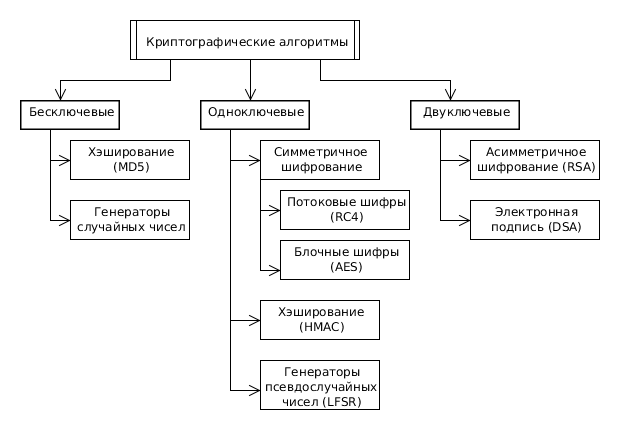
\includegraphics[width=\linewidth]{./imgs/CA_classification.png}

\end{frame}

\begin{frame}
  \frametitle{Симметричная криптография}

  \begin{block}{Протокол передачи зашифрованного сообщения}
  \begin{enumerate}
    \item{Алиса и Боб выбирают систему шифрования}
    \item{Алиса и Боб выбирают ключ}
    \item{Алиса шифрует открытый текст с использованием алгоритма шифрования и ключа}
    \item{Алиса посылает шифрованное сообщение Бобу}
    \item{Боб дешифрует шифротекст с использованием того же алгоритма и ключа}
  \end{enumerate}
  \end{block}
\end{frame}


\begin{frame}
  \frametitle{Симметричная криптография (продолжение)}

  \begin{block} {Недостатки симметричных криптосистем}
  \begin{itemize}
    \item{Распределение ключей должно проводиться в секрете.}
    \item{Если ключ скомпрометирован, то злоумышленник может создавать ложные сообщения от лица одной из сторон протокола.}
    \item{Если каждая пара пользователей сети использует отдельный ключ, то общее количество ключей быстро 
          возрастает с ростом числа пользователей.}
          \note{100 пользователей --- 4950 ключей}
  \end{itemize}
  \end{block}
\end{frame}

\begin{frame}
  \frametitle{Односторонняя функция}
  \note{Не является протоколом, но является центральным понятием в криптографии с открытым ключом}
  \define{Односторонняя функция (англ. one-way function, OWF)} {это функция, которая легко вычисляется для
         любого входного значения, но трудно найти аргумент по заданному значению функции}

  Зная $x$ легко легко вычислить $f(x)$, но по известному $f(x)$ нелегко вычислить $x$.
  \note{Легко разбить тарелку на 1000 различных кусочков, но непросто собрать её обратно из кусочков}
  \note{Математически строгого доказательства существования односторонних функций нет, нет
        и реальных свидетельств возможности их построения}

  \vspace{1\baselineskip}

  \define{Односторонняя функция с потайным входом (англ. trapdoor function)} {это функция, которая легко вычисляется
  в одном направлении, но трудно вычисляется в обратном без специальной информации (секрета), называемой «лазейкой» или «потайным входом»}
\end{frame}

\begin{frame}
  \frametitle{Криптография с открытыми ключами}
  \begin{block}{Особенности}
    \begin{itemize}
      \item{Протокол использует два различных ключа --- один открытый $K_{pub}$ и один закрытый $K_{priv}$.}
      \item{Открытый ключ $K_{pub}$ может быть общедоступным. Любой может зашифровать сообщение, используя этот ключ.}
      \item{Закрытый ключ $K_{priv}$ держится в секрете. Только владелец закрытого ключа может расшифровать
        сообщение, зашифрованное открытым ключом.}
      \item{Математическая основа - односторонняя функция с потайным входом.}
    \end{itemize}
  \end{block}
  \note{Симметричный алгоритм - сейф. Каждый должен знать код, чтобы открыть его.
  Алгоритм с открытым ключом - почтовый ящик. Каждый может положить сообщение, открыть ящик может только владелец.}
\end{frame}


\begin{frame}
  \frametitle{Криптография с открытыми ключами}
  \begin{block}{Посылка сообщения}
    \begin{enumerate}
      \item{Алиса и Боб согласовывают криптосистему с открытыми ключами.}
      \item{Боб посылает Алисе свой открытый ключ.}
      \item{Алиса шифрует свое сообщение и отправляет его Бобу.}
      \item{Боб расшифровывает сообщение Алисы с помощью своего закрытого ключа.}
    \end{enumerate}
  \end{block}
\end{frame}


\begin{frame}
  \frametitle{Криптография с открытыми ключами}
  \begin{block}{Недостатки}
    \begin{itemize}
      \item{Алгоритмы с открытыми ключами работают медленно.}
      \item{Криптосистемы с открытыми ключами уязвимы по отношению к некоторым видам атак.}
    \end{itemize}
  \end{block}
\end{frame}


\begin{frame}
  \frametitle{Криптографическая хеш-функция}

  \define {Хеш-функция} {функция, которая получает на вход строку переменной длины (прообраз) и преобразует её в строку
           фиксированной, обычно меньшей длины}
  \begin{block} {Свойства идеальной криптографической хеш-функции}
    \begin{itemize}
      \item{Значение хеш-функции легко вычислимо для любого прообраза}
      \item{Практически невозможно подобрать прообраз для заданного значения хеш-функции}
      \item{Практически невозможно найти два различных прообраза с одинаковым хешем}
    \end{itemize}
  \end{block}
\end{frame}


\begin{frame}
  \frametitle{Применения криптографической хеш-функции}

  \begin{itemize}
    \item{Проверка целостности файла или сообщения}
    \item{Верификация паролей}
    \item{Идентификация данных}
    \item{Получение новых ключей или паролей из имеющихся}
    \item{Проверка подлинности сообщений}
    \item{Цифровая подпись}
  \end{itemize}
\end{frame}


\begin{frame}
  \frametitle{Цифровая подпись с помощью криптографии с открытым ключом}

  \begin{block} {Протокол}
    \begin{enumerate}
      \item{Алиса шифрует документ своим закрытым ключом, таким образом подписывая его}
      \item{Алиса посылает подписанный документ Бобу}
      \item{Боб расшифровывает документ, используя открытый ключ Алисы, таким образом проверяя подпись}
    \end{enumerate}
  \end{block}
\end{frame}


\begin{frame}
  \frametitle{Использование криптографической хеш-функции в цифровой подписи}

  \begin{block} {Протокол}
    \begin{enumerate}
      \item{Алиса получает значение криптографической хеш-функции для документа}
      \item{Алиса шифрует это значение своим закрытым ключом, таким образом подписывая документ}
      \item{Алиса посылает Бобу документ и подписанное значение хеш-функции}
      \item{Боб получает значение криптографической хеш-функции для документа, присланного Алисой. Затем,
            он расшифровывает подписанное значение хеш-функции с помощью открытого ключа Алисы. Если подписанное
            значение хеш-функции совпадает с рассчитанным, то подпись правильна.}
    \end{enumerate}
  \end{block}
\end{frame}


\begin{frame}
  \frametitle{Генерация случайных и псевдослучайных последовательностей}

  \begin{itemize}
    \item{Встроенные в компиляторы и стандартные библиотеки реализации генератора псевдослучайных чисел вовсе не случайны}
    \item{Криптографическая псевдослучайная последовательность должна быть непредсказуема}
  \end{itemize}
\end{frame}


\begin{frame}
  \frametitle{Список литературы}

  \begin{itemize}
    \item{Брюс Шнайер ``Прикладная криптография``}
  \end{itemize}
\end{frame}

\end{document}
